%!TEX root = ./intern_report.tex

\newpage
\subsection{Building Wallie: A Hardware Platform for Data Collection and Deployment}

\paragraph{}
The Robotics and Autonomous Systems Group of DATA61 is about field robotics. Therefore, it is not sufficient to demonstrate a concept theoretically or just by simulations. Instead, the members are expected to demonstrate our systems and results in complex real world environments.

\paragraph{}
Therefore, we needed a robot platform on which we can collect data and perform our tests. However, the available platforms of CSIRO were all in use for bigger projects. Hence we were requested to build a robot platform based on Pololu Wild Thumper chassis. This platform was previously assembled by our seniors: Isuru and Tharindu. However, as we describe below, we had to change almost every component of that to create a new robot to suit our specific needs. Our friend from Chile named this robot Wallie, in reference to the Wall-E movie and the fact our robot was initially built to follow walled hallways.

\begin{figure}[H]
    \centering
    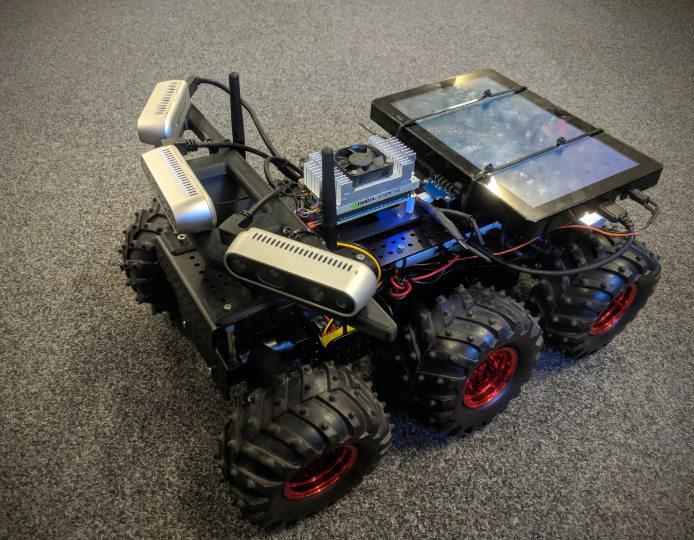
\includegraphics
        [width=10cm]
        {figures/wallie.PNG}
    \caption{Wallie: The Robot \label{Fig:wallie}}\vspace{-4mm}
\end{figure}

\paragraph{}
Firstly, we need a way to fix cameras in the robot for data collection and testing. I sketched a small camera rig to hold three Intel Realsense cameras, each facing: center, left and right at 30 degree angles from center. Samith Ashan, my coworker helped designed it in solidworks. That, a platform for the Jetson TX2 board and a holder for the Li-ion battery were then 3D printed. 

\subsubsection{Power Distribution System}

\begin{figure}[H]
    \centering
    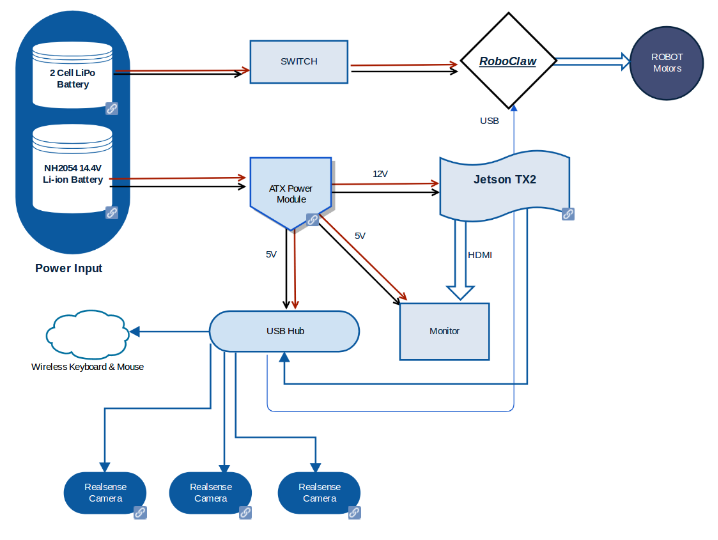
\includegraphics
        [width=13cm]
        {figures/wallie_hardware.PNG}
    \caption{Wallie: Hardware Hierarchy }\vspace{-4mm}
\end{figure}

\paragraph{}
We then designed a power distribution system for the robot, to deliver power from two batteries to all the sensors and actuators. We consulted Dr. Navinda and Mr. James Brett and came of with the following system. A 3 cell Li-Po delivers power to the Roboclaw Motor Controller, to which six 12V, 2.5D high torque motors are connected through a switch and a fuse (to prevent damage to the motor controller in case if the motors start stalling, as it happened once). The cameras and IMU are powered through an active USB hub. The USB hub LCD display and NVIDIA Jetson TX2 are powered through a robust power supply (12V, 5V) which is connected through a switch to the 7.4V Li-ion battery. Having two separate power sources for high-level and low-level systems helped through decoupling by reducing the chances of power failures from one network damaging the component in the other.

\paragraph{}
We documented the design of the robot in CSIRO's confluence wiki pages, so that fellow researchers can use it in the future for their own activities. Most of our time in CSIRO (about 75\%) was spent in building and debugging the robot platform. 


\subsubsection*{NVIDIA Jetson TX2}

Jetson TX2 is 

% Table: Jetson
\begin{table}[H]
    \begin{center}
        \caption {NVIDIA Jetson TX2 Specifications} \label{tab:jetson}
        \begin{tabular}{|| r || l ||}    
            \hline
            GPU             & 256 CUDA cores of Pascal Architecture \\
            \hline
            CPU             & HMP Dual Denver 2/2 MB L2 + Quad ARM® A57/2 MB L2 \\
            \hline
            Memory          & 8 GB 128 bit LPDDR4, 59.7 GB/s \\
            \hline
            Data storage    & 32 GB \\
            \hline 
            USB             & USB 3.0 \\
            \hline 
            Connectivity    & Gigabit Ethernet, 802.11ac WLAN, Bluetooth \\
            \hline   
        \end{tabular}    
    \end{center}
\end{table}

% Image: Jetson
\begin{figure}[H]
    \centering
    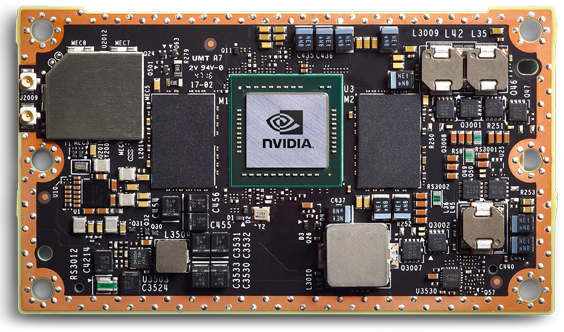
\includegraphics
        [width=8cm]
        {figures/jetson.png}
    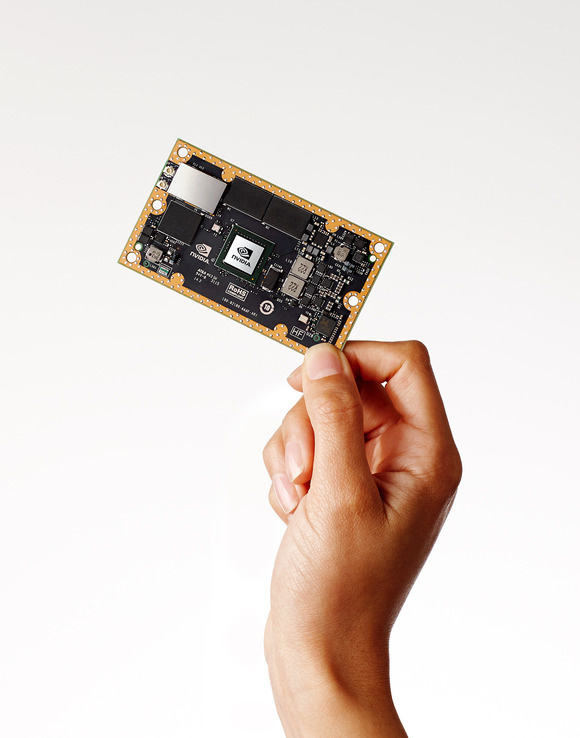
\includegraphics
        [height=5cm]
        {figures/jetson_scale.jpg}
    \caption{NVIDIA Jetson TX2 }\vspace{-4mm}
\end{figure}



\subsubsection*{Intel Realsense Depth Camera D435}

% Image: Realsense
\begin{figure}[H]
    \centering
    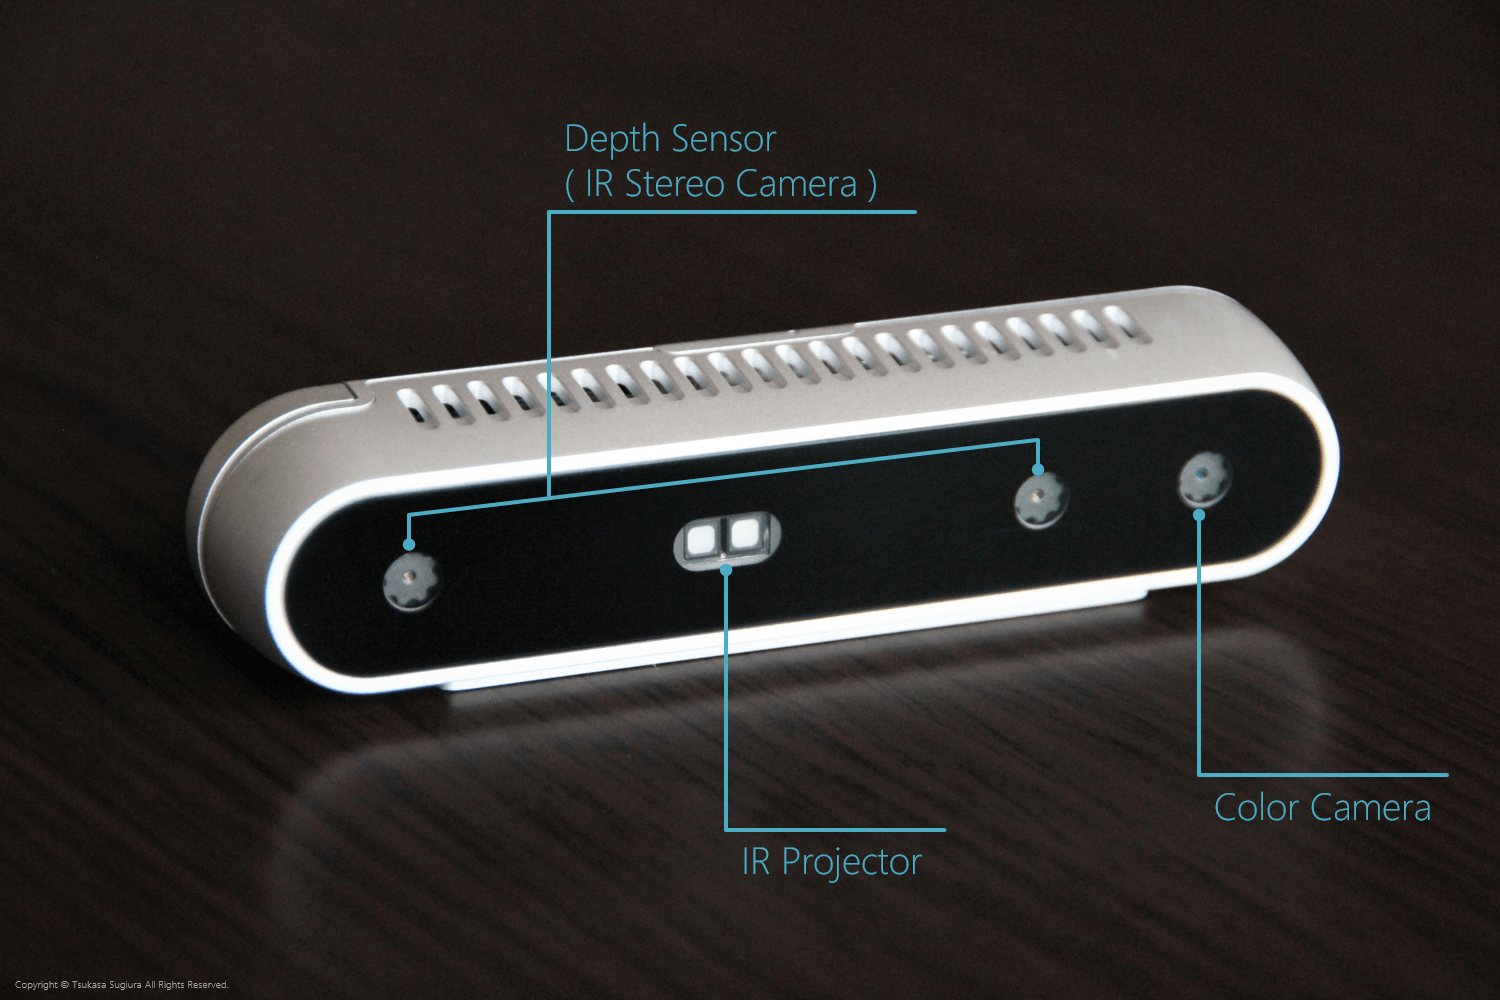
\includegraphics
        [width=12cm]
        {figures/realsense.png}
    \caption{Intel Realsense D435}\vspace{-4mm}
\end{figure}

% Table: Realsense
\begin{table}[H]
    \begin{center}
        \caption {Intel Realsense D435 Specifications} \label{tab:realsense}
        \begin{tabular}{|| r || l ||}
            \hline
            Depth FOV (Horz, Vert, Diag)	& 85.2\degree x 58\degree x 94\degree (+/- 3\degree) \\
            \hline
            Depth Stream Output Resolution	& Up to 1280 x 720 \\
            \hline
            Depth Stream Output Frame Rate	& Up to 90 fps \\
            \hline
            Maximum Range	                & Approx.10 meters \\
            \hline
            RGB   FOV (Horz, Vert, Diag)	& 69.4\degree x 42.5\degree x 77\degree (+/- 3\degree) \\
            \hline
            RGB   FOV (Horz, Vert, Diag)	& 1920 x 1080 at 30 fps \\
            \hline
            Connectors	                    & USB 3.0 Type - C \\
            \hline
        \end{tabular}    
    \end{center}
\end{table}


\subsubsection*{Roboclaw Motor Controller}

% Table: Roboclaw
\begin{table}[H]
    \begin{center}
        \caption {Pololu Roboclaw Motor Controller Specifications} \label{tab:roboclaw}
        \begin{tabular}{|| r || l ||}    
            \hline
            Motor channels              &   2   \\
            \hline
            Control interface           &	USB; TTL serial (2-way), RC pulses; PWM\\
            \hline
            Minimum operating voltage   &	6 V \\
            \hline
            Maximum operating voltage   &	34 V \\
            \hline
            Continuous output current per channel   &	30 A \\
            \hline
            Peak output current per channel         &	60 A \\
            \hline   
        \end{tabular}    
    \end{center}
\end{table}

% Image: 2 motor controllers
\begin{figure}[H]
    \centering
    \begin{minipage}{.5\textwidth}
        \centering
        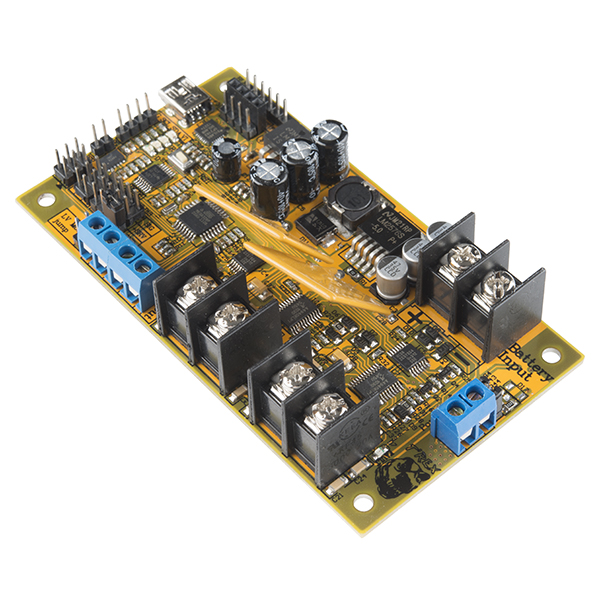
\includegraphics[width=\linewidth]{figures/trex.jpg}
        \captionof{figure}{TREX Motor Controller}
        \label{fig:test1}
    \end{minipage}%
    \begin{minipage}{.5\textwidth}
        \centering
        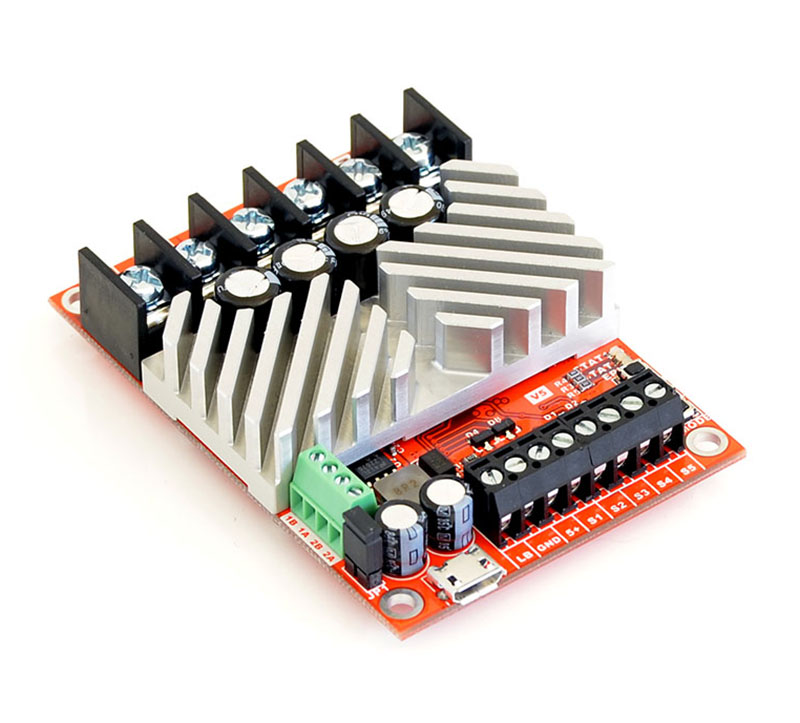
\includegraphics[width=\linewidth]{figures/roboclaw.jpg}
        \captionof{figure}{Roboclaw Motor Controller}
        \label{fig:test1}
    \end{minipage}
\end{figure}



\subsubsection*{Problems Faced and Solutions}